 
%%%%%%%%%%%%%%%%%%%%%%%%%%%%%%%%%%%%%%%%%%%%%%%%%%%%%%%%%%%%
%%  This Beamer template was created by Cameron Bracken.
%%  Anyone can freely use or modify it for any purpose
%%  without attribution.
%%
%%  Last Modified: January 9, 2009
%%

\documentclass[xcolor=x11names,compress]{beamer}
% \documentclass[xcolor=x11names,compress,handout]{beamer}

%% General document %%%%%%%%%%%%%%%%%%%%%%%%%%%%%%%%%%
\usepackage{graphicx}
\usepackage{verbatim}
\newenvironment{metaverbatim}{\verbatim}{\endverbatim}
\usepackage{tikz}
\usetikzlibrary{decorations.fractals}
%%%%%%%%%%%%%%%%%%%%%%%%%%%%%%%%%%%%%%%%%%%%%%%%%%%%%%


%% Beamer Layout %%%%%%%%%%%%%%%%%%%%%%%%%%%%%%%%%%
\useoutertheme[subsection=false,shadow]{miniframes}
\useinnertheme{default}
\usefonttheme{serif}
\usepackage{palatino}
\usepackage{wrapfig}
\setbeamerfont{title like}{shape=\scshape}
\setbeamerfont{frametitle}{shape=\scshape}

\setbeamercolor*{lower separation line head}{bg=DeepSkyBlue4} 
\setbeamercolor*{normal text}{fg=black,bg=white} 
\setbeamercolor*{alerted text}{fg=red} 
\setbeamercolor*{example text}{fg=black} 
\setbeamercolor*{structure}{fg=black} 
 
\setbeamercolor*{palette tertiary}{fg=black,bg=black!10} 
\setbeamercolor*{palette quaternary}{fg=black,bg=black!10} 

\renewcommand{\(}{\begin{columns}}
\renewcommand{\)}{\end{columns}}
\newcommand{\<}[1]{\begin{column}{#1}}
\renewcommand{\>}{\end{column}}
%%%%%%%%%%%%%%%%%%%%%%%%%%%%%%%%%%%%%%%%%%%%%%%%%%



\usepackage{pgf,pgfarrows,pgfnodes,pgfautomata,pgfheaps,pgfshade}
\usepackage{amsmath,amsfonts,amssymb,graphicx,epsfig}
\usepackage[latin1]{inputenc}
\usepackage{colortbl}
\usepackage[english]{babel}
\usepackage{graphics}
\usepackage{graphicx,amsbsy,amsmath,amsfonts}
%\usepackage{algorithm}
\usepackage{times}
\usepackage{listings}
\usepackage{fancyvrb}
\usepackage{multicol}
\usepackage{listings}
% \usepackage{tabu}
% \usepackage{animate}
%\usepackage{capt-of}
% \newtheorem{assumption}{Assumption}

\def\ds{\displaystyle}
\newcommand{\dive}{\nabla\cdot}
\newcommand{\bD}{{\bf D}}
\newcommand{\bu}{{\bf u}}
\newcommand{\bv}{{\bf v}}
\newcommand{\bw}{{\bf w}}
\newcommand{\bU}{{\bf U}}
\newcommand{\bV}{{\bf V}}
\newcommand{\bX}{{\bf X}}
\newcommand{\mbD}{{\mathbb{D}}}

\newcommand{\be}{{\bf e}}
\newcommand{\bz}{{\bf z}}
\newcommand{\bx}{{\bf x}}
\newcommand{\bff}{{\bf f}}
\newcommand{\bd}{{\bf d}}
\newcommand{\bo}{{\bf }}
\newcommand{\bnu}{\boldsymbol\nu}
\newcommand{\bn}{\boldsymbol n}
\newcommand{\btau}{\boldsymbol\tau}
\newcommand{\bsigma}{\boldsymbol\sigma}
\newcommand{\bpsi}{\boldsymbol\psi}
\newcommand{\bphi}{\boldsymbol\phi}
\def\Web{\mbox{\text{We}}} 
\def\Fro{\mbox{\text{Fr}}}  
\def\Rey{\mbox{ \text{Re}}}  
\def\Wei{\mbox{ \text{Wi}}} 
 
 
 \newcommand{\mbT}{{\mathbb{T}}}
\newcommand{\mbS}{{\mathbb{S}}}
 
\newcommand{\mbI}{{\mathbb{I}}} 
\newcommand{\mbR}{{\mathbb{R}}}
\newcommand{\mbP}{{\mathbb{P}}}
\newcommand{\mbB}{{\mathbb{B}}}
 \newcommand{\bp }{\boldsymbol{+}}
 \newcommand{\bop }{\boldsymbol{\oplus}}
\newcommand{\bomg}{\boldsymbol\omega}
 
 

\definecolor{darkblue}{rgb}{0,0,1}
\definecolor{darkgreen}{rgb}{0,0.6,0}
\definecolor{darkbrown}{rgb}{0,0.9,0.8}
\definecolor{darkblue&}{rgb}{0,0,1}
\definecolor{red}{rgb}{1,0,0}
\definecolor{lightblue}{rgb}{.9,1,1}



\title{\textcolor{darkgreen}{ParMooN \\ (Parallel Mathematical Object Oriented Numerics)}}

\author[Prof. Sashikumaar Ganesan]
{
\textbf{Sashikumaar Ganesan}
\\ 
    {\tiny\textit{jointly with ...}}
    \\ Sangeeta Yadav,
}

\institute[IISc, India]
{
Computational Mathematics Group\\
Department of Computational and Data Sciences\\
Indian Institute of Science, Bangalore, India\\  
}

\date{Version 1.0 (2019)}
     
\begin{document}

\begin{frame}

% \begin{center}
% \Large
% \bf
%  WCCM XII -- APCOM VI -- SEOUL 2016
% \end{center}
% \vspace{-5mm}
 \titlepage
\end{frame}
\footnotesize

% \begin{frame}
% %   \frametitle{Outline}
%   \tableofcontents[part=1]
%  %\tableofcontents[part=1,pausesections]
% \end{frame}


%\AtBeginSection[]
%{
% \begin{frame}<beamer>
%\frametitle{Outline}
% \tableofcontents[current,currentsection]
% \tableofcontents[part=1]
%\end{frame}
%}


\part<presentation>{Main Talk}
 
\section[Mathematical Model]{Introduction to FEM}
%   \subsection{Motivation}
     \frametitle{Motivation}
 
 \onslide<+->
%\begin{block}{Fluid Flow Models}
%\begin{itemize}
%  \item Advanced approaches exists for fixed domains
%\onslide<+->
%  \item Situation changes if the {\color<2>[rgb]{1,0,0}{domain moves} }
%        with {\color<2>[rgb]{1,0,0}{large deformation} }
%  \onslide<+->
%  \item More complicate if the {\color<3>[rgb]{1,0,0}{boundary is priori unknown}}
%        and/or the   {\color<3>[rgb]{1,0,0}{surface tension}} and other effects
%        are considered  
%\end{itemize}
%\end{block}
  \onslide<+->
\begin{block}{Objective}
\begin{itemize}
  \item To develop a robust and reliable algorithms for 
         {\color<4>[rgb]{1,0,0}incompressible flows in moving domains}
\end{itemize}
\end{block}
  \subsection[Model Problem]{Fluid Flow That We Considered}
 % \input{sub03}

  \subsection[Mathematical Model]{Mathematical Model}


\section[Numerical Schemes]{Numerical Schemes}
  \subsection{Weak Formulation}
%\begin{frame}[Content..]
  	
%\end{frame}

\begin{frame}{Version Control System}
	
	It is a software that helps software developers to work together and maintain a complete history of their work.The functions of a VCS are as follows: 
\begin{wrapfigure}{r}{0.25\textwidth}
		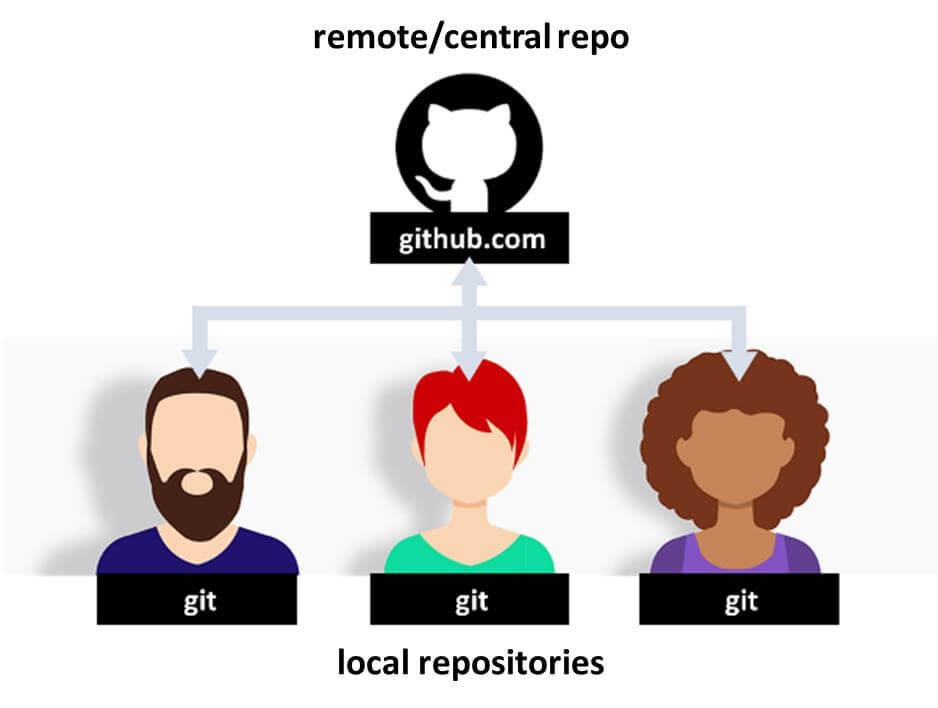
\includegraphics[width=0.28\textwidth]{s13.jpg}
\end{wrapfigure}
	\begin{enumerate}
	\item Allows developers to work simultaneously.
	\item Does not allow overwriting each others changes.
	\item Maintains a history of every version.
	\end{enumerate}
	
	Types of VCS : 
	\begin{enumerate}
	\item Centralized version control system (CVCS).
	\item Distributed/Decentralized version control system (DVCS).
	\end{enumerate}
	Git is a distributed version-control system for tracking changes in source code during software development.
	%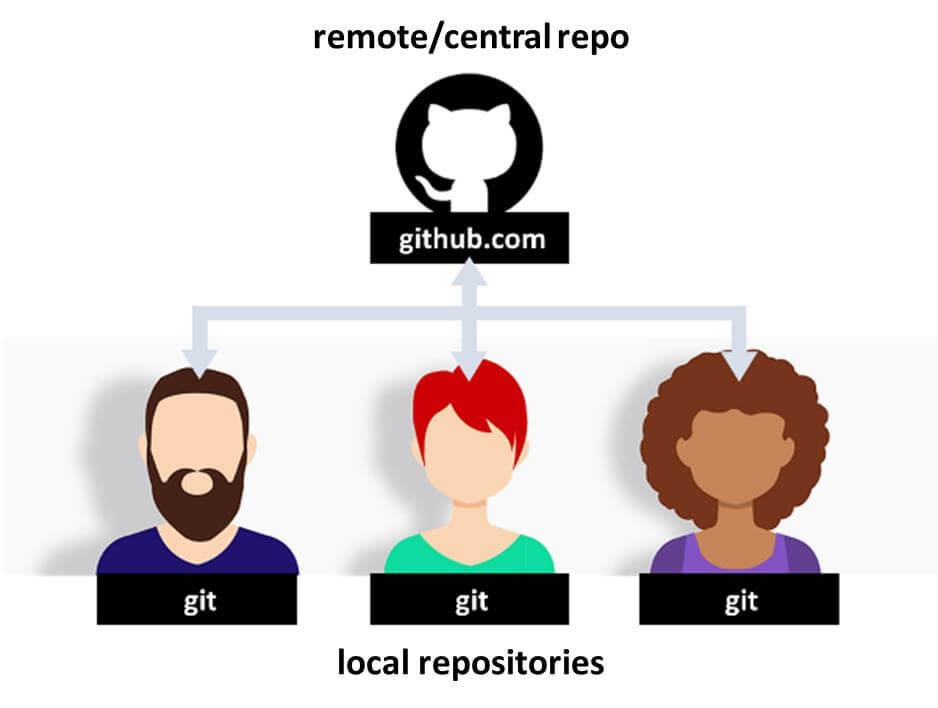
\includegraphics[width = 0.5\textwidth,height = 0.5\textheight]{s13.jpg}
\end{frame}
%\begin{frame}{Advantages of Git}
%	\begin{enumerate}
%		\item Free and open source
%		
%	\end{enumerate}
%	\end{frame}
\begin{frame}{Installation}
	\begin{itemize}
		\item 	\textbf{Fedora :} yum install git 
		\item \textbf{Ubuntu :} sudo apt-get install git
		\item \textbf{Windows :} Just go to http://git-scm.com/download/win
		\item Set your username and password.
		\begin{itemize}
		\item \text{\$ git config --global user.name "John Doe"}
		\item \text{\$ git config --global user.email johndoe@example.com}
	\end{itemize}
	\end{itemize}
\end{frame}
\begin{frame}
	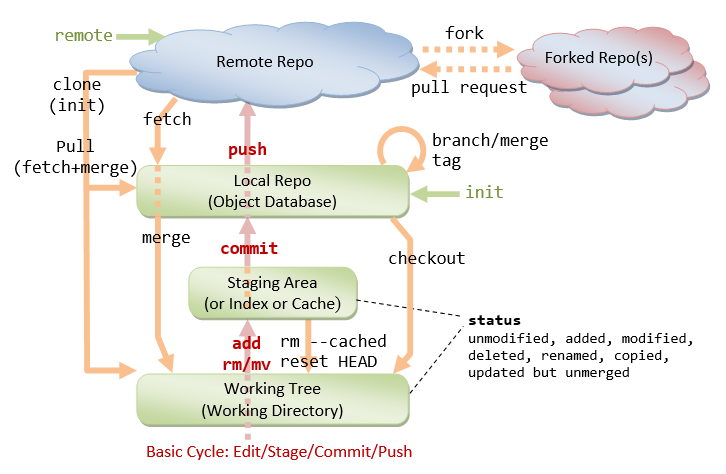
\includegraphics[width = \textwidth,height = 0.7\textheight]{s11.png}
\end{frame}

\begin{frame}{The lifecycle of the status of your files}
	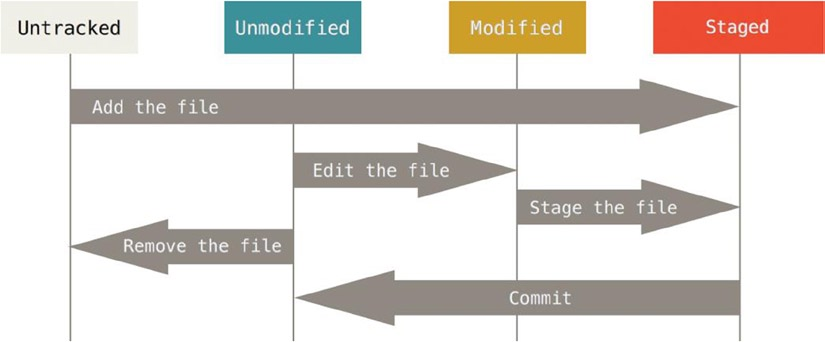
\includegraphics[width = \textwidth,height = 0.5\textheight]{s9.png}
\end{frame}

%\begin{frame}{The lifecycle of the status of your files}
%	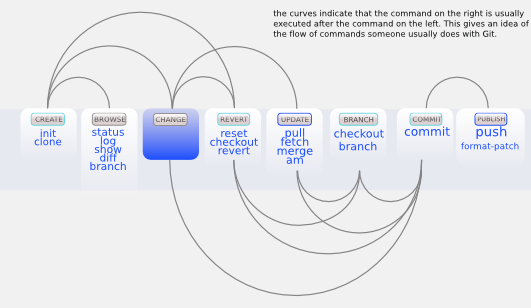
\includegraphics[width = \textwidth,height = 0.7\textheight]{s10.png}
%\end{frame}
%\begin{frame}
%	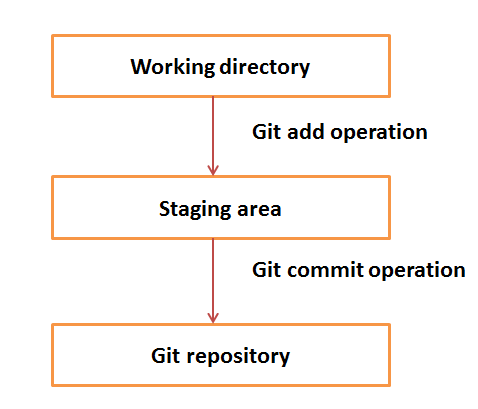
\includegraphics[width = \textwidth,height =0.8 \textheight]{s8.png}
%\end{frame}
%\begin{frame}{Commands}
%	\begin{itemize}
%		\item Glossary
%		\item Branch
%		\item Checkout
%		\item Cherry-picking
%		\item Clone
%		\item Fetch
%		\item Fork
%		\item HEAD
%		\item Index
%		\item Master
%		\item Merge
%		\item Origin
%		\item Pull/Pull Request
%		\item Push
%		\item Remote
%		\item Repository
%		\item Stash
%	\end{itemize}
%\end{frame}
%\begin{frame}{Commands}
%		\textbf{git fetch :}
%		The git fetch command communicates with a remote repository and fetches down all the information that is in that
%		repository that is not in your current one and stores it in your local database.\newline
%		\textbf{git pull:}
%		The git pull command is basically a combination of the git fetch and git merge commands, where Git will fetch
%		from the remote you specify and then immediately try to merge it into the branch you?re on.\newline
%		\textbf{git push:}
%		The git push command is used to communicate with another repository, calculate what your local database has
%		that the remote one does not, and then pushes the difference into the other repository.
%		\end{frame}
\begin{frame}{Commands}
\textbf{git init [repository name]		}	\newline	This command is used to start a new repository.	\newline	\newline
\textbf{git clone [url]		}	\newline	This command is used to obtain a repository from an existing URL.\newline	\newline
\textbf{ git add [file]}\newline
This command adds a file to the staging area.\newline	\newline
\textbf{git add *		}	\newline	This command adds one or more to the staging area.\newline\newline
\textbf{git commit -m "[ Type in the commit message]"}	\newline	This command records or snapshots the file permanently in the version history.	\newline	\newline
\textbf{git commit -a}	\newline
This command commits any files you've added with the git add command and also commits any files you've changed since then.\newline \newline

\end{frame}
\begin{frame}{Commands}
\textbf{git diff}	\newline	This command shows the file differences which are not yet staged.	\newline	\newline
\textbf{git diff -staged}	\newline	This command shows the differences between the files in the staging area and the latest version present.	\newline	\newline
\textbf{git diff [first branch] [second branch]		}	\newline	This command shows the differences between the two branches mentioned.	\newline	\newline
\textbf{git reset}	\newline	This command unstages the file, but it preserves the file contents.	\newline	\newline
\textbf{git reset [commit]		}	\newline	This command undoes all the commits after the specified commit and preserves the changes locally.	\newline	\newline
\textbf{git reset -hard [commit]}	\newline	This command discards all history and goes back to the specified commit.	\newline	\newline

\end{frame}
\begin{frame}{Commands}
\textbf{git status		}	\newline	This command lists all the files that have to be committed.	\newline	\newline
\textbf{git rm [file]		}	\newline	This command deletes the file from your working directory and stages the deletion.	\newline	\newline
\textbf{git log		}	\newline This command is used to list the version history for the current branch.
\newline	\newline
\textbf{git log -follow[file]}	\newline	This command lists version history for a file, including the renaming of files also.	\newline	\newline
\textbf{git show [commit]		}	\newline	This command shows the metadata and content changes of the specified commit.	\newline	\newline
	\end{frame}
	\begin{frame}{Commands}
		\textbf{ git tag [commitID]		}	\newline	This command is used to give tags to the specified commit.	\newline	\newline
		\textbf{git branch		}	\newline	This command lists all the local branches in the current repository.	\newline	\newline
		\textbf{git branch [branch name]}	\newline "This command creates a new branch."	\newline	\newline
		\textbf{git branch -d [branch name]		}	\newline	This command deletes the feature branch.	\newline	\newline
		\textbf{git checkout [branch name]		}	\newline	This command is used to switch from one branch to another.	\newline	\newline
		\textbf{git checkout -b [branch name]		}	\newline	This command creates a new branch and also switches to it.	\newline	\newline
		\textbf{git merge [branch name]		}	\newline	This command merges the specified branch?s history into the current branch.	\newline	\newline
		
	\end{frame}
		\begin{frame}{Commands}
		\textbf{git remote add [variable name] [Remote Server Link]		}	\newline	This command is used to connect your local repository to the remote server.	\newline	\newline
		\textbf{git push [variable name] master		}	\newline	This command sends the committed changes of master branch to your remote repository.	\newline	\newline	
		\textbf{ git push [variable name] [branch]		}	\newline	This command sends the branch commits to your remote repository.	\newline	\newline
		\textbf{git push -all [variable name]}	\newline	This command pushes all branches to your remote repository.	\newline	\newline
		\textbf{git push [variable name] :[branch name]		}	\newline	This command deletes a branch on your remote repository.
			\newline	\newline
		\textbf{git pull [Repository Link]		}	\newline	This command fetches and merges changes on the remote server to your working directory.	\newline	\newline
	\end{frame}
%\end{frame}	
\section{Cmake}
\begin{frame}{Cmake}
	\begin{itemize}
		\item It is an extensible, open-source system that manages the build process in an operating system and in a compiler-independent manner. 
		\item It can generate a native build environment that will compile source code, create libraries, generate wrappers and build executables in arbitrary combinations
		\item Users can configure builds through a GUI
		\item It supports static and dynamic library builds. 
		\item It helps to manage and build your source codes effectively
	\end{itemize}
	\end{frame}
\begin{frame}{	Source and Build Trees		}
	\begin{itemize}				
		\item	The Source Tree contains:
		\begin{itemize}
		\item CMake input files (CMakeLists.txt)
		\item Program source files (hello.cxx)
		\end{itemize}
		\item	The Binary Tree (build tree) contains:
			\begin{itemize}			
		\item Native build system files (hello.dsp)
		\item Program libraries and executables (hello.exe)
		\end{itemize}			
		\item Source and Binary trees may be:
		\begin{itemize}
		\item In the same directory (in-source build)
		\item In different directories (out-of-source build)
		\end{itemize}
	\end{itemize}	
\end{frame}	
\begin{frame}
	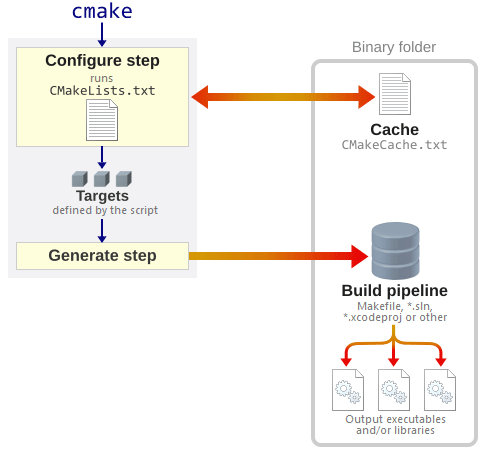
\includegraphics[width = 0.7\textwidth,height = 0.7\textheight]{s13.png}
\end{frame}
\begin{frame}{Installation}
	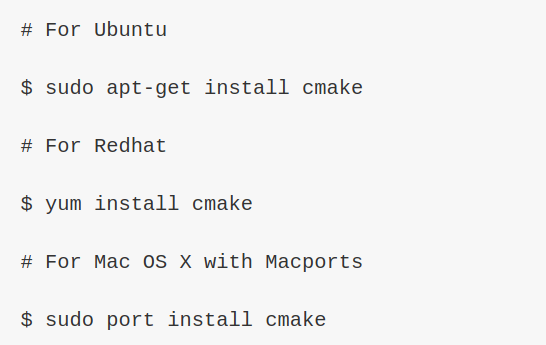
\includegraphics[width = 0.7\textwidth,height = 0.4\textheight]{s14.png}
%	\text{cmake_minimum_required (VERSION 2.6)}
%\text{project (Tutorial)}
%\text{add_executable(Tutorial tutorial.cxx)}
	\end{frame}			
\begin{frame}{The CMake Cache}
\begin{itemize}
\item Represents build configuration
\item Populated by CMake code
\item Stored in CMakeCache.txt at top of build
\item Entries have a type to help the GUI
\item Holds global information for CMake code
\item Updated by CMake configuration phase
	\end{itemize}
\end{frame}

\begin{frame}{Cmake files in ParMooN}
	\text{/ParMooN/ParMooN/CMakeLists.txt}\newline 
	\text{/ParMooN/ParMooN/UserConfig.cmake}
\end{frame}

\begin{frame}{Different uses of Cmake in ParMooN}
	\begin{itemize}
		\item Include main program 
		\item Mention the output directory
		\item Select the architecture type
		\item Select the parallel type
		\item Select the Operating system
		\item Link static and dynamic libraries
	\end{itemize}
\end{frame}
\begin{frame}{VS code}
	\begin{itemize}
		\item Developed by Microsoft for Windows, Linux and macOS.
		\item Includes support for debugging, embedded Git control and GitHub, syntax highlighting, intelligent code completion, snippets, and code refactoring.
		\item It is highly customizable, allowing users to change the theme, keyboard shortcuts, preferences, and install extensions that add additional functionality. \item It is free and open source and released under the permissive MIT License.
	\end{itemize}
\end{frame}

\begin{frame}{Basic Layout}
	\begin{enumerate}
		\item Editor - The main area to edit your files. 
		\item Side Bar - Contains different views like the Explorer to assist you while working on your project.
		\item Status Bar - Information about the opened project and the files you edit.
		\item Activity Bar - Located on the far left-hand side, this lets you switch between views and gives you additional context-specific indicators, like the number of outgoing changes when Git is enabled.
		\item Panels - You can display different panels below the editor region for output or debug information, errors and warnings, or an integrated terminal. Panel can also be moved to the right for more vertical space.
	\end{enumerate}
\end{frame}
\begin{frame}
	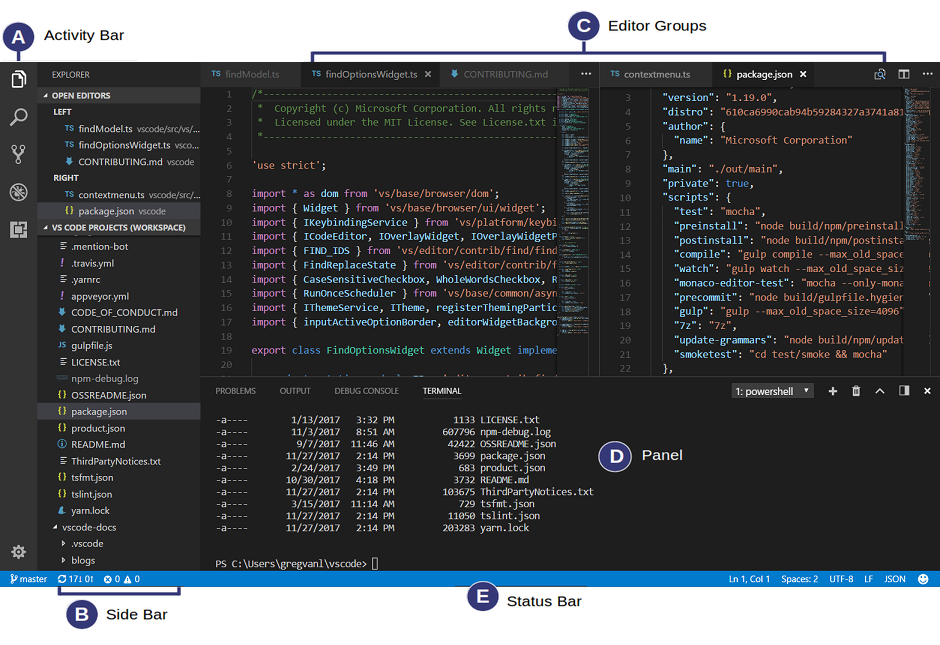
\includegraphics[width = \textwidth, height = \textheight]{s1.png}
\end{frame}

\begin{frame}{Side by side editing}
	\begin{enumerate}
		\item Alt click on a file in the Explorer.
		\item Ctrl+\ to split the active editor into two.
		\item Open to the Side (Ctrl+Enter) from the Explorer context menu on a file.
		\item Click the Split Editor button in the upper right of an editor.
		\item 	Drag and drop a file to any side of the editor region.
		\item 		Ctrl+Enter (macOS: Cmd+Enter) in the Quick Open (Ctrl+P) file list.
	\end{enumerate}
\end{frame}  
%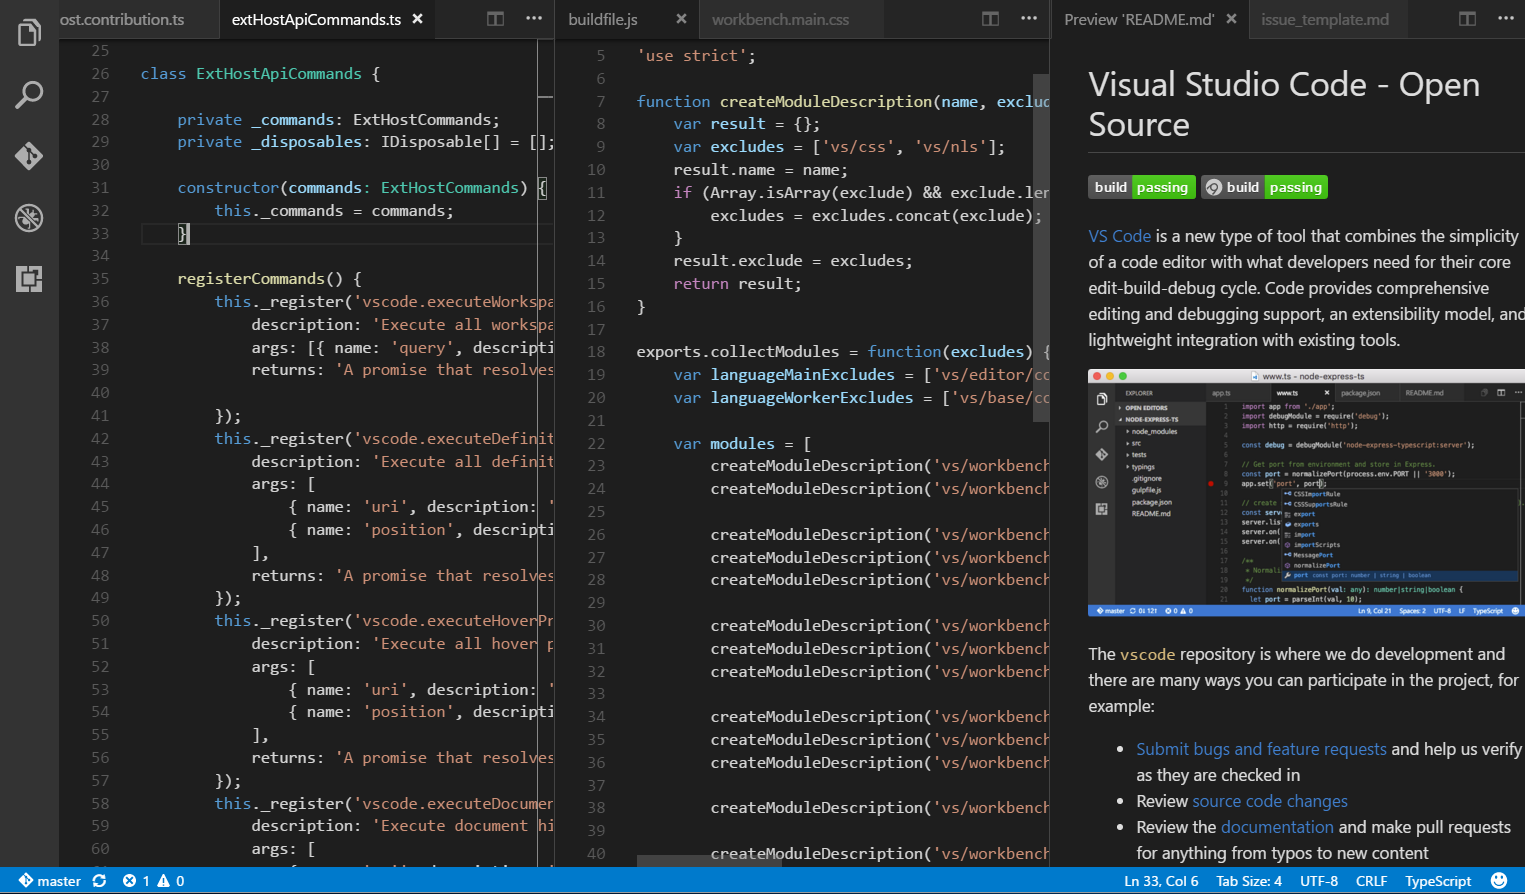
\includegraphics[width = \textwidth, height = \textheight]{s2.png}
% \begin{center}
% \Large
% \bf
%  WCCM XII -- APCOM VI -- SEOUL 2016
% \end{center}
% \vspace{-5mm}
%	\titlepage

\begin{frame}
	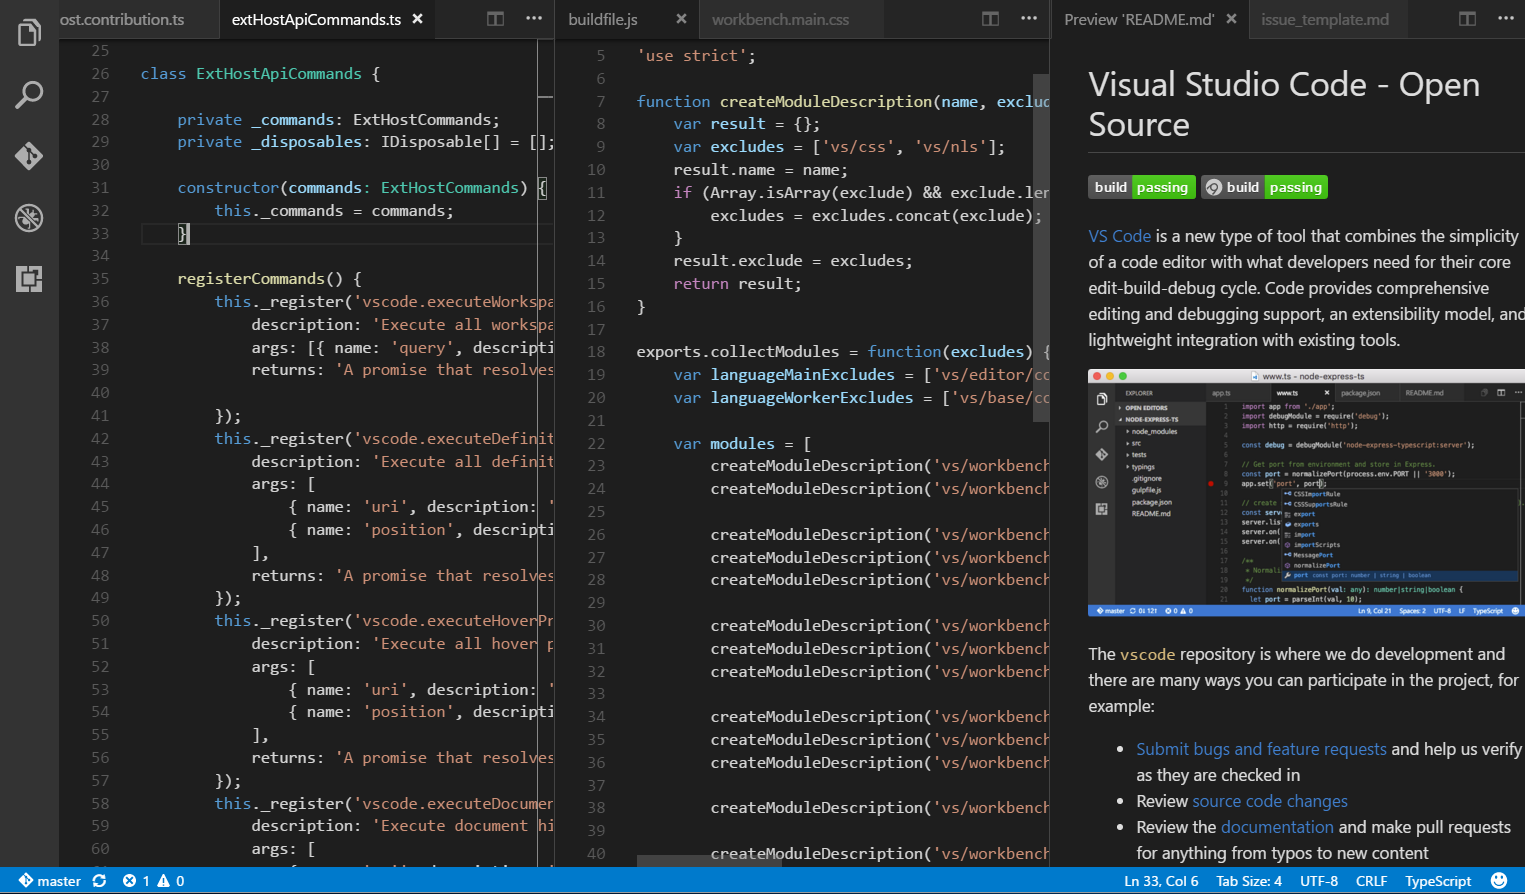
\includegraphics[width = \textwidth, height = \textheight]{s2.png}
\end{frame}
\begin{frame}{Language specific editor settings}
	Customize the editor by language:
	\begin{itemize}
		\item Run the global command Preferences: Configure Language Specific Settings (command id: workbench.action.configureLanguageBasedSettings) from the Command Palette (Ctrl+Shift+P) which opens the language picker. 
		\item Selecting the required language, opens the Settings editor with the language entry where you can add applicable settings.
	\end{itemize}
\end{frame}

%\end{metaverbatim}
\end{document}
